\documentclass{beamer}
%\documentclass[handout]{beamer}
%\usepackage{pgfpages}
%\pgfpagesuselayout{2 on 1}[a4paper,border shrink=5mm]

\usepackage{verbatim}
\usepackage{amssymb}
\usepackage{amsmath}

\mode<presentation>
{
  \usetheme{Singapore}  %Warsaw}  %CambridgeUS}
  
  \setbeamercovered{transparent}
  }


\usepackage[english]{babel}
\usepackage[latin1]{inputenc}
\usepackage{times}
\usepackage[T1]{fontenc}
\newcommand{\bs}{\boldsymbol}
\newcommand{\mb}{\mathbf}
\newcommand{\x}{\mathbf{x}}
\newcommand{\X}{\mathbf{X}}
\newcommand{\y}{\mathbf{y}}
\newcommand{\Y}{\mathbf{Y}}

\title[Descriptive Regression with a Binary Covariate] {Lecture 1\\Descriptive Regression with a Binary Covariate}


\date{August 24, 2023}

\AtBeginSection[]
{
  \begin{frame}<beamer>
    \frametitle{Outline}
    \tableofcontents[currentsection,currentsubsection]
  \end{frame}
}


\AtBeginSubsection[]
{
  \begin{frame}<beamer>
    \frametitle{Outline}
    \tableofcontents[currentsection,currentsubsection]
  \end{frame}
}

\begin{document}

\begin{frame}
  \titlepage
\end{frame}




\begin{frame}
  \frametitle{Outline}
  \tableofcontents
 
\end{frame}

\frame{
\frametitle{What are descriptive statistics?}

\begin{itemize}
\item Descriptive statistics are summaries of the data we have. \pause
\item The data we have might be a sample (e.g., an exit poll) or it might be the whole population (e.g., administrative vote counts), sometimes known as a census. \pause
\item Having the whole population is becoming more common in the era of Big Data.\pause
\item Note: if you are interested in the causal effects of a treatment (a drug, a policy, etc.), you can never really have the whole population (we will discuss this in a few weeks).
\end{itemize}

}

\frame{
\frametitle{What makes a good summary?}

What are the two things that make a good summary?

\vspace{.5cm}

\visible<2>{
From the google definition:
\begin{enumerate}
\item brief
\item includes main points
\end{enumerate}}


}

\frame{
\frametitle{What makes a good descriptive statistic?}

\begin{enumerate}
\item brief: at most a few numbers \pause
\item includes main points: \pause
\begin{itemize}
\item sufficient to describe main characteristics of the data
\begin{itemize}
\item there is a technical definition of sufficiency that I can discuss in office hours for those interested
\end{itemize} \pause
\item minimizes the information lost by reducing the data
\begin{itemize}
\item I'm using ``information'' in a loose sense here, will formalize a bit later
\item reducing the data means taking the data, which are often represented by $n*v$ numbers (with $n$ the number of observations and $v$ the number of variables) and reducing to a descriptive statistic that is represented by a few numbers.
\end{itemize}
\end{itemize}
\end{enumerate} \pause

Enough forest. Trees (examples) are coming!


}

\frame{
\begin{center}
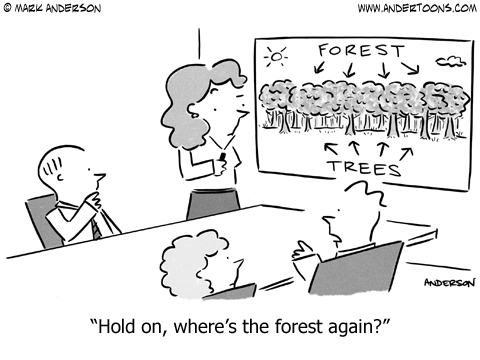
\includegraphics[scale=.4]{figs/forest_tree_cartoon}
\end{center}
It is easy in a statistics class to focus on the specifics. I want you to remember why we are doing what we are doing.

}


\section{Univariate Descriptive Statistics}





\frame{
\frametitle{Univariate Example: SCOTUS data}

\begin{itemize}
\item Data on 27 justices from the Warren (`53 - `69), Burger (`69 - `86), and Rehnquist (`86 - `05) courts \pause
\item Data can be interpreted as a census for the 1953 - 2005 era.  \pause
\item One Variable: Percentage of votes in liberal direction for each justice in civil liberties cases
\end{itemize}

\begin{table}[h]
\begin{center}
\begin{tabular}{r|r}
Justice & CLlib   \\
\hline
Black & 74.2  \\
Reed & 33.3 \\
\vdots & \vdots \\
Thomas & 25.6 \\
\hline
\end{tabular}
\end{center}
\end{table}


}

\frame{
\frametitle{Describing Univariate Data}

\begin{figure}[ht] \centering
        \scalebox{.4}{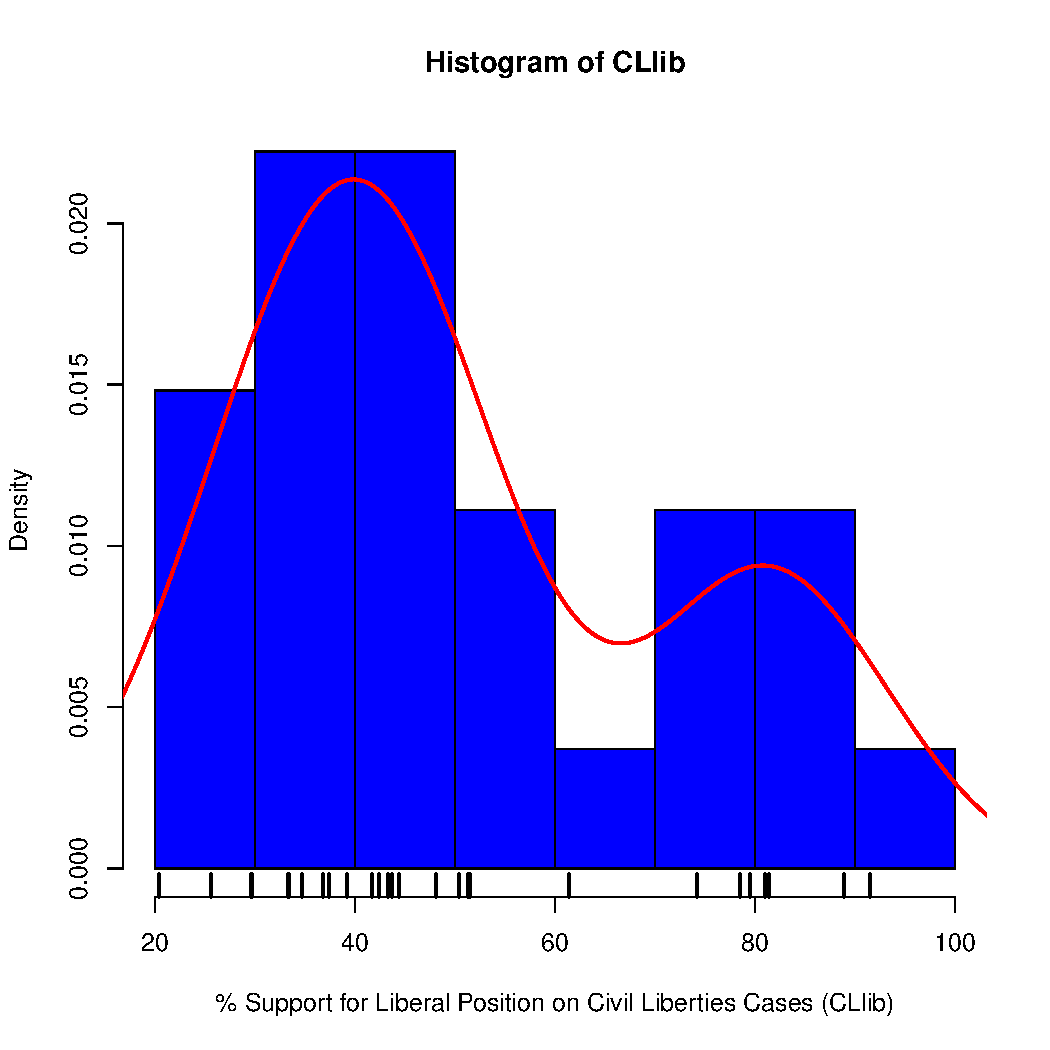
\includegraphics{figs/CLhist.pdf}}
\end{figure}


}


\frame{
\frametitle{Description/Summarization}

\begin{itemize}
\item Even for univariate data, we may want to focus on one or two characteristics of the population instead of describing it in its entirety. \pause
\item We typically focus on measures of center and spread.\pause
\item We will discuss the rational for this over the coming weeks.
\end{itemize}
}


\frame{
\frametitle{Univariate Activity}

\begin{figure}[ht] \centering
        \scalebox{.4}{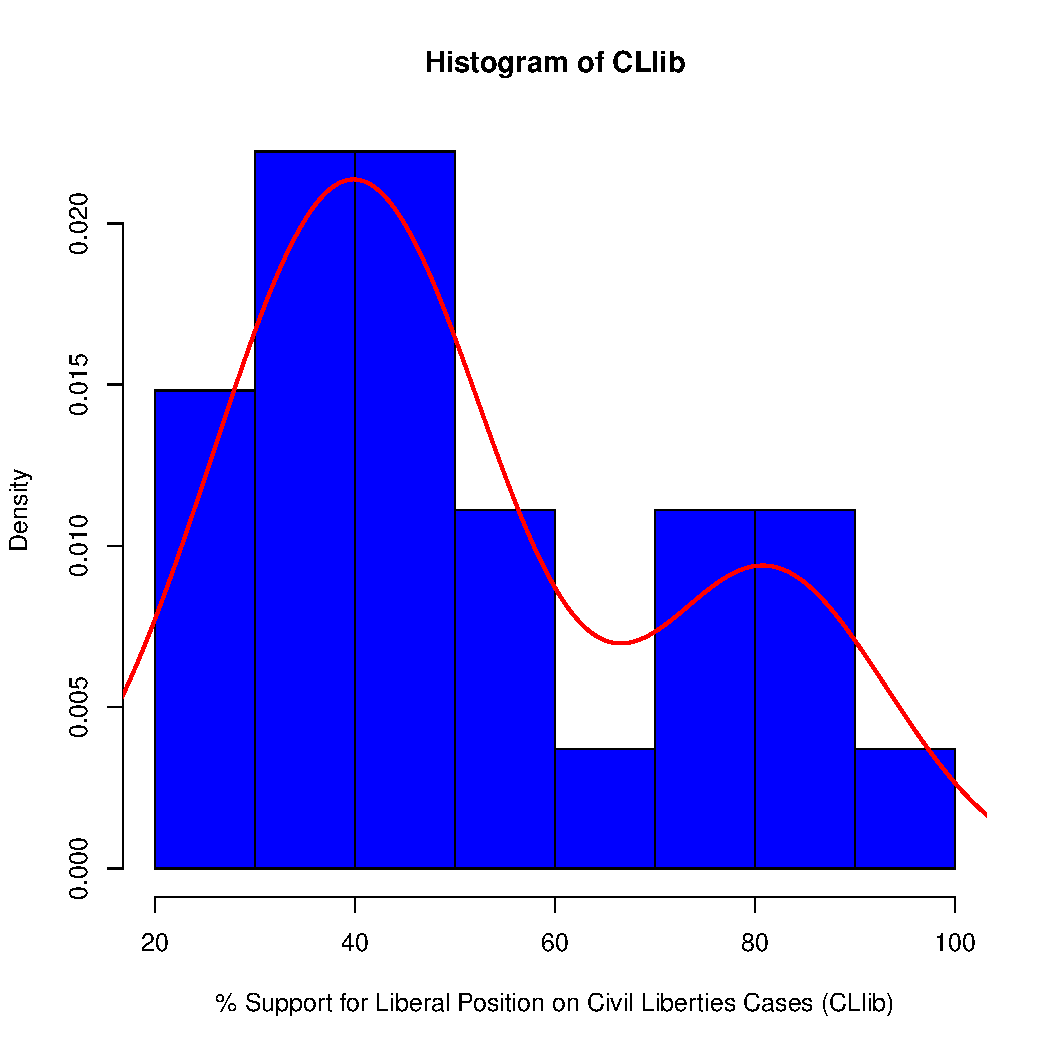
\includegraphics{figs/CLhistAct.pdf}}
\end{figure}
\centering Find the rough location of the mean and median.
}

\frame{
\frametitle{Univariate Activity Solution}

\begin{figure}[ht] \centering
        \scalebox{.4}{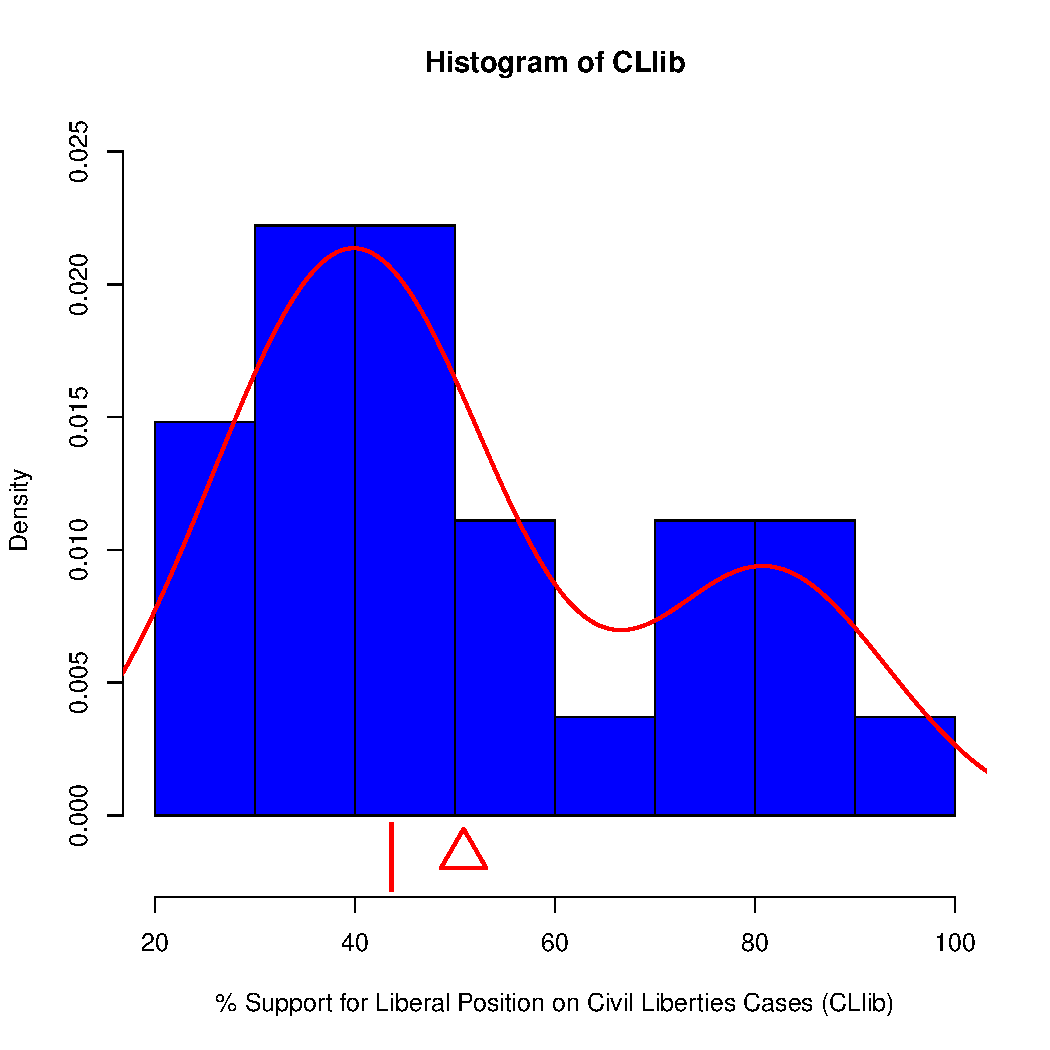
\includegraphics{figs/CLhistActSol.pdf}}
\end{figure}

}

\frame{
\frametitle{Mean/Median Discussion}

In pairs, discuss what the mean and median represent in the context of the CLib variable for these justices. What does it mean for the mean to be larger than the median in this context?

}

\frame{
\frametitle{Mean as a balance point}
\begin{center}
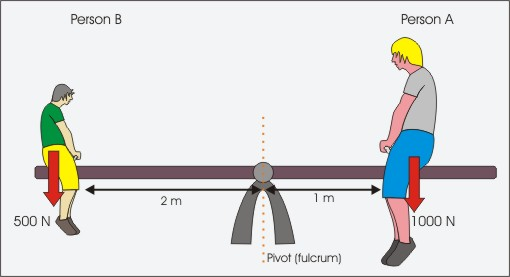
\includegraphics[scale=.5]{figs/seesaw}
\end{center}
}


\frame{
\frametitle{Choosing a descriptive statistic}

How might we choose between these descriptive statistics?

\begin{enumerate}
\item brief: at most a few numbers \pause
\item includes main points: \pause
\begin{itemize}
\item sufficient to describe main characteristics of the data
\item minimizes the information lost by reducing the data
\end{itemize}
\end{enumerate} 

}




\frame{
\frametitle{A Least Squares Summary}

Suppose we want to pick a single number ($m$) for the middle of the data that summarizes all the values for $y$, by minimizing the sum of squared residuals (i.e., least squares).
$$
SSR(\tilde{m}) = \sum_{i=1}^N (y_i - \tilde{m})^2.
$$
\pause

Activity: Using calculus, derive the least squares estimator
\begin{enumerate}
  \item Calculate the derivative of $SSR$ with respect to $\tilde{m}$
  \item Set the derivative equal to 0
  \item Solve for $m$
\end{enumerate}

}



\frame{
\frametitle{The Objective Function for SSR CLlib}
\begin{figure}[ht] \centering
        \scalebox{.4}{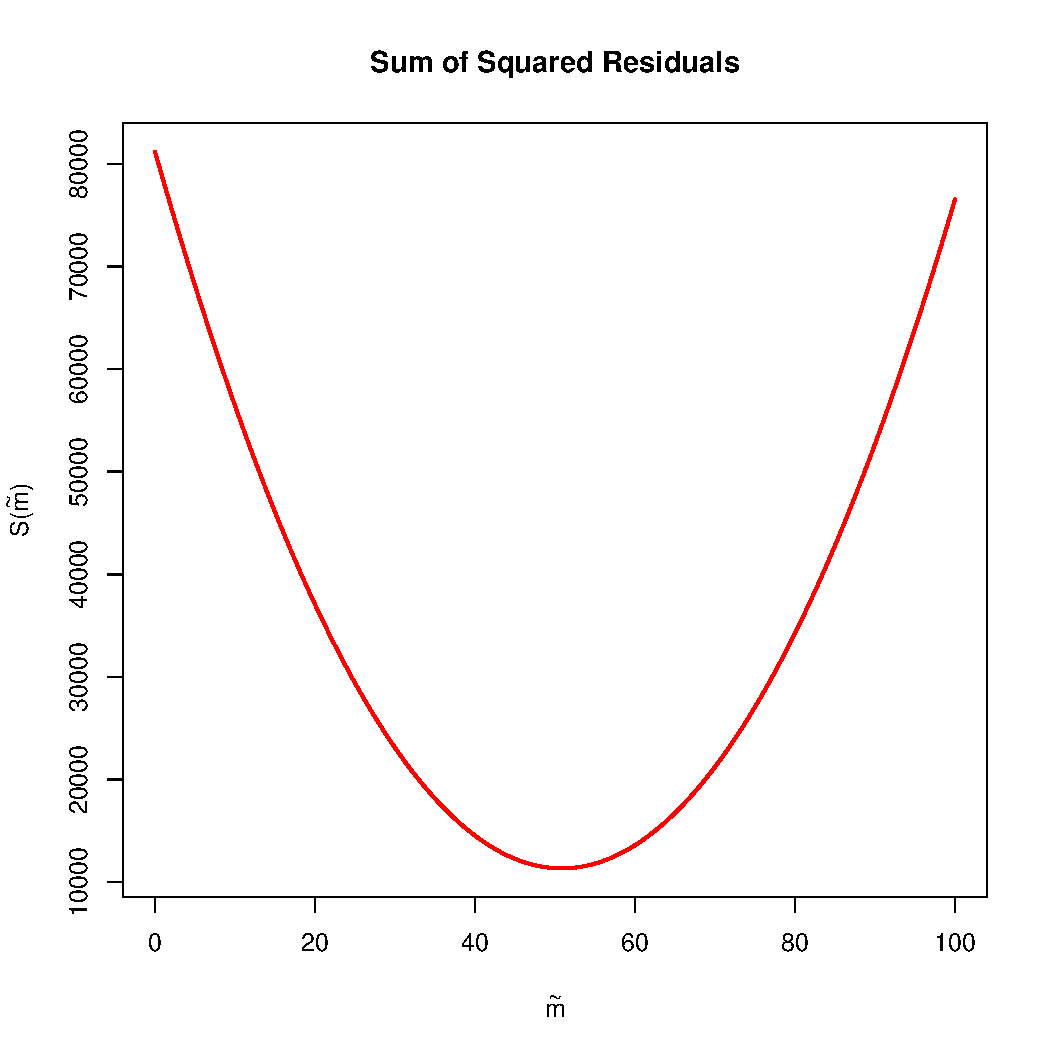
\includegraphics{figs/objectiveFunction1.pdf}}
\end{figure}

}

\frame{

\begin{enumerate}
\item \begin{align*}
SSR(\tilde{m}) 
  &= \sum_{i=1}^N (y_i -
  \tilde{m})^2\\
  &= \sum_{i=1}^N (y_i^2 - 2 y_i \tilde{m} + \tilde{m}^2)
\end{align*} 
 $$
\frac{\partial SSR(\tilde{m})}{\partial
  \tilde{m}} = \sum_{i=1}^N (-2 y_i + 2 \tilde{m})
$$
\end{enumerate}


\vspace{3cm}
}

\frame{
\frametitle{The Slope of the Tangent Line for SSR CLlib}
\begin{figure}[ht] \centering
        \scalebox{.4}{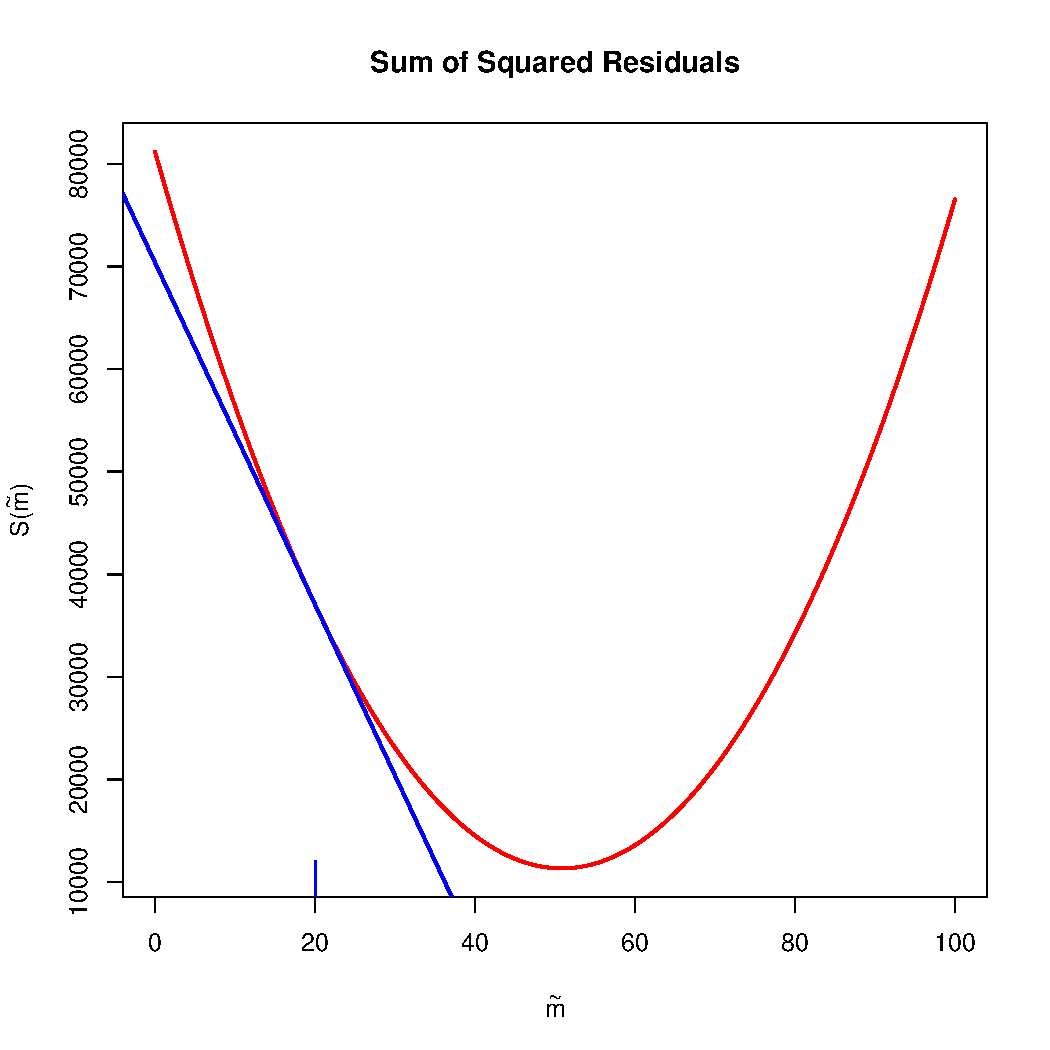
\includegraphics{figs/objectiveFunction2.pdf}}
\end{figure}

}

\frame{
\frametitle{The Slope of the Tangent Line for SSR CLlib}
\begin{figure}[ht] \centering
        \scalebox{.4}{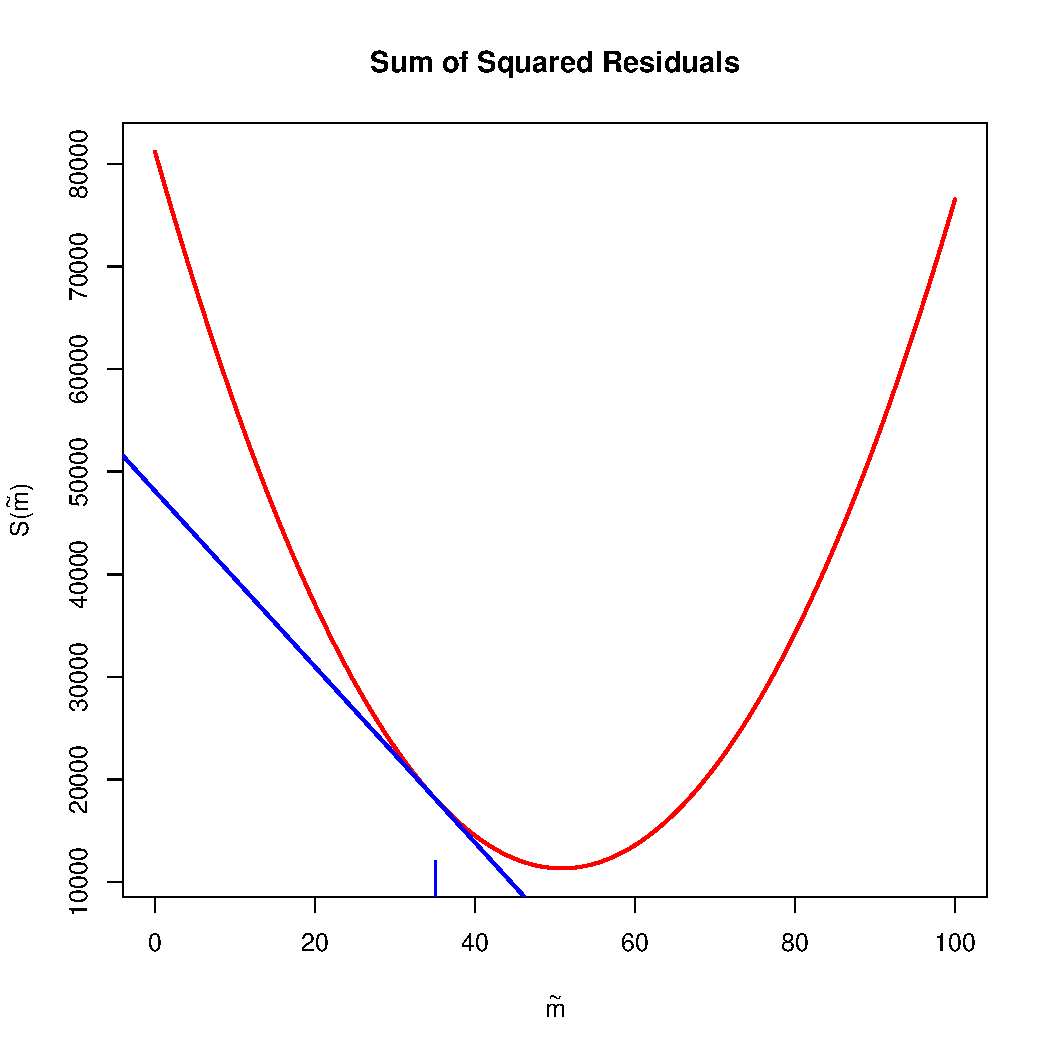
\includegraphics{figs/objectiveFunction3.pdf}}
\end{figure}

}

\frame{
\frametitle{The Slope of the Tangent Line for SSR CLlib}
\begin{figure}[ht] \centering
        \scalebox{.4}{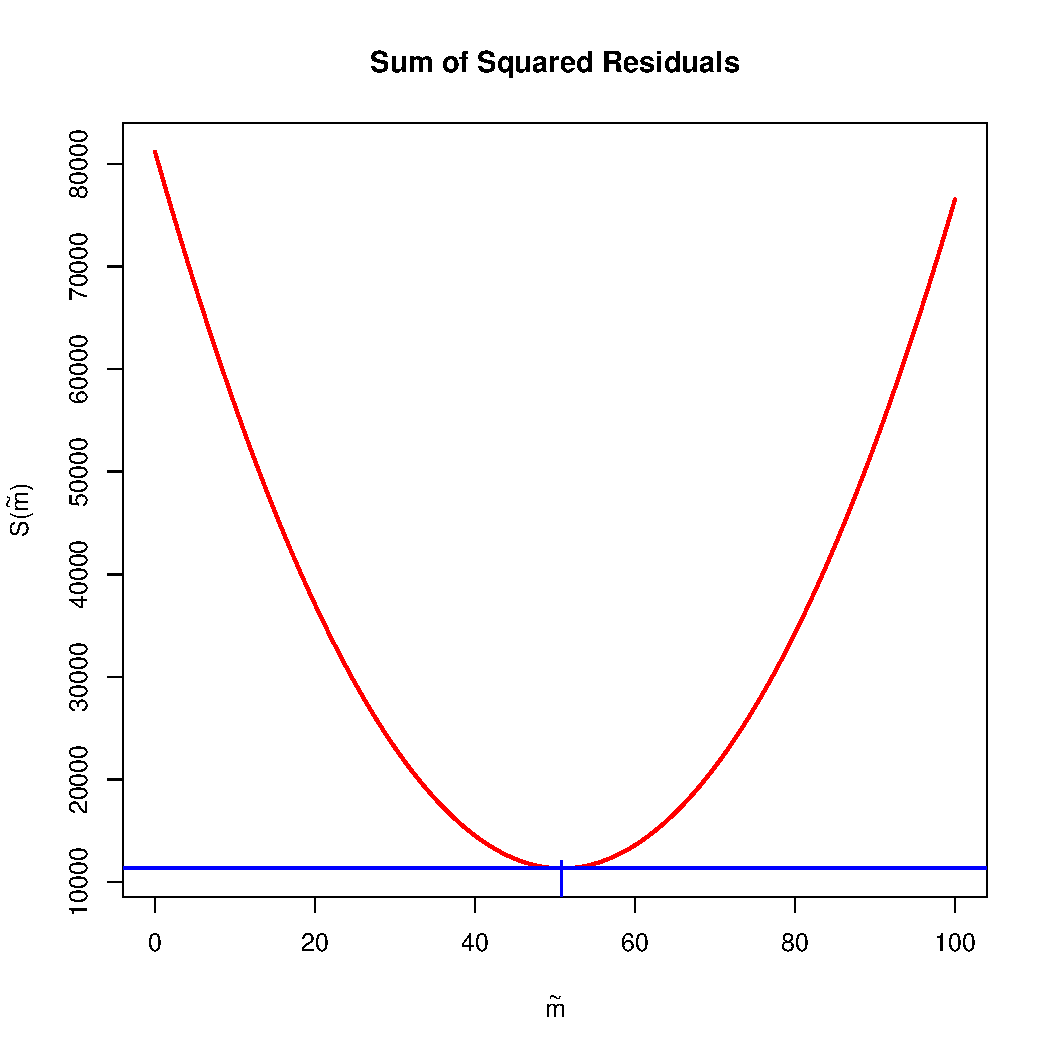
\includegraphics{figs/objectiveFunction4.pdf}}
\end{figure}

}


\frame{

\begin{enumerate}
\item \begin{align*}
SSR(\tilde{m}) 
  &= \sum_{i=1}^N (y_i -
  \tilde{m})^2\\
  &= \sum_{i=1}^N (y_i^2 - 2 y_i \tilde{m} + \tilde{m}^2)
\end{align*} 
 $$
\frac{\partial S(m)}{\partial
  \tilde{m}} = \sum_{i=1}^N (-2 y_i + 2\tilde{m})
$$

\item $$
0 = \sum_{i=1}^N (-2 y_i + 2 m)
$$
\item $$
m = \frac{1}{N}\sum_{i=1}^N  y_i 
$$
\end{enumerate}
\vspace{.1cm}
\centering Therefore, the mean is a least squares summary.

}


\frame{
\frametitle{A Least Absolute Value Summary}

Suppose we want to pick a single number ($m$) for the middle of the data that summarizes all the values for $y$, by minimizing the sum of absolute deviations.
$$
SAV(\tilde{m}) = \sum_{i=1}^N |y_i - \tilde{m}|.
$$
\pause


\begin{itemize}
  \item Why is this harder to solve?
  \item Any guesses?
\end{itemize}

}


\frame{
\frametitle{Why we focus on means}

\begin{itemize}
\item Means often provide a ``good'' summary of the data (and it is relatively easy to tell when they provide bad summaries).  \pause
\item The properties of means are relatively easy to describe.  \pause
\item Randomized experiments only identify mean causal effects (as do regression and matching when the appropriate assumptions hold).
\end{itemize}

}

\frame{
\frametitle{Variance and Standard Deviation}

\begin{itemize}
\item Mean is the least squares predictor in terms of SSR.
\item How small is ``least'' (i.e., how much spread around the mean)?
\item Variance and Standard Deviation are useful transformations of SSR for the mean.
\end{itemize} \pause

Variance
\begin{align*}
S^2 &= \frac{\sum_{i=1}^N (y_i-\bar{y})^2}{N-1} \\ 
&=  \frac{SSR}{N-1}
\end{align*} \pause

Standard Deviation
\begin{align*}
S &= \sqrt{S^2}
\end{align*}

}

\frame{
\frametitle{Mean and Standard Deviation}

\begin{figure}[ht] \centering
        \scalebox{.4}{
\includegraphics{figs/CLhistMSD.pdf}}
\end{figure}


}

\frame{
\frametitle{Variance as turning force}

\begin{center}
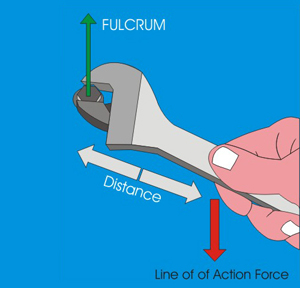
\includegraphics[scale=.5]{figs/turning_effect_01}
\end{center}
}

\frame{
\frametitle{Why variance and standard deviation?}

\begin{itemize}
\item Natural measures of accuracy for means.  \pause
\item Means and standard deviations are sufficient to describe the distribution of normally distributed data. \pause
\item For non-normal data, means and standard deviations provide information via Chebyshev's inequality and other concentration inequalities. 
\end{itemize}

}

\frame{
\frametitle{Normally Shaped Histograms}

\begin{center}
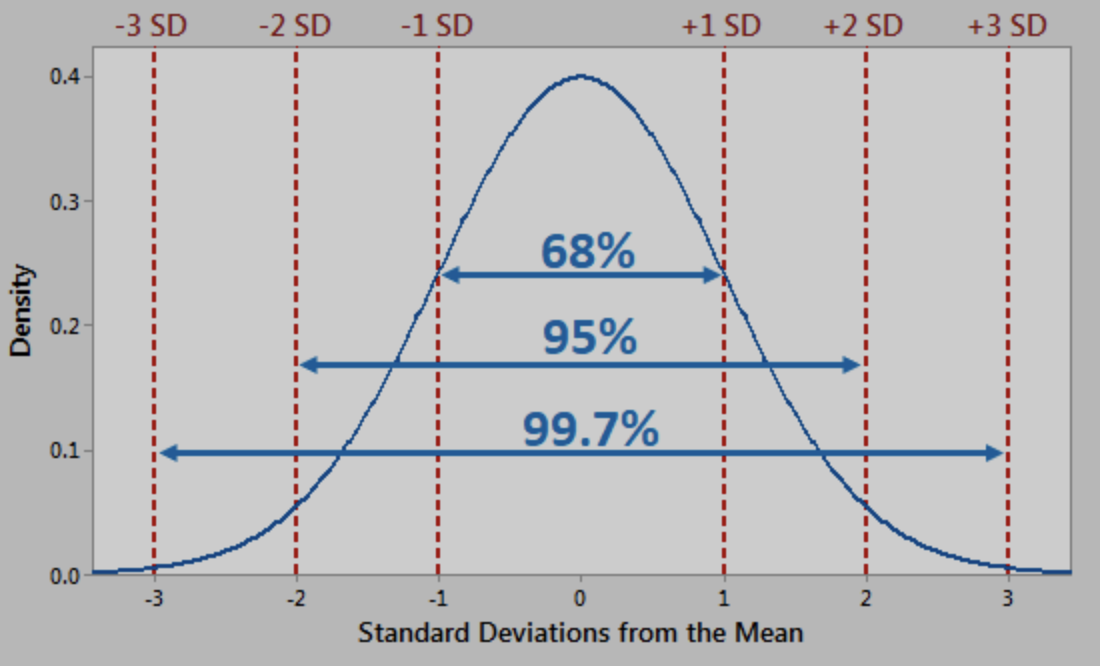
\includegraphics[scale=.5]{figs/empiricalRule.png}
\end{center}
}

\frame{
\frametitle{Chebyshev for Non-normal Histograms}

\begin{center}
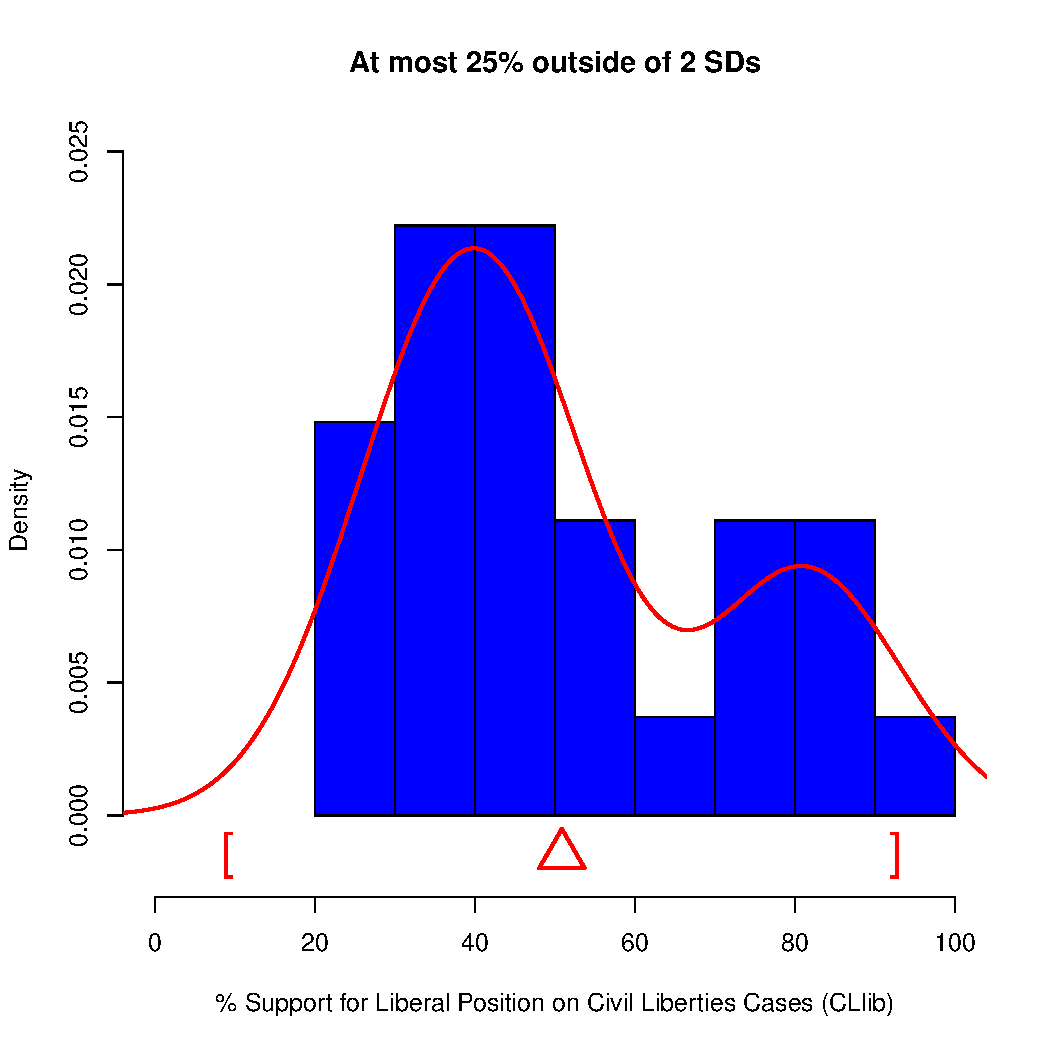
\includegraphics[scale=.4]{figs/Chebyshev.pdf}
\end{center}
}


\frame{
\frametitle{Special Case: Binary Variables}

\begin{table}[h]
\begin{center}
\begin{tabular}{r|r}
Justice & Underrepresented Group   \\
\hline
Black & 0  \\
\vdots & \vdots\\
Marshall & 1 \\
Burger & 0 \\
\vdots & \vdots \\
O'Connor & 1 \\
Scalia & 0 \\
\vdots & \vdots \\
Thomas & 1 \\
\hline
Proportion & 3/27\\
\end{tabular}
\end{center}
\end{table}

}


\frame{
\frametitle{Mean and Variance for UR Group Variable}


\begin{align*}
\bar{y} &= \frac{1}{N}\sum_{i=1}^{N} y_i \\
&= \frac{0 + \dots+ 1+ 0 + \dots + 1 + 0 + \dots+ 1}{27} \\
&= \frac{3}{27}\\
&\\
S^2 &= \frac{\sum_{i=1}^{N} (y_i-\bar{y})^2}{N-1} \\ 
&= \frac{(0-.11)^2 + \dots+ (1-.11)^2}{27-1}  \\ 
&=  \left(\frac{27}{27-1}\right)[\bar{y} \cdot(1-\bar{y})]
\end{align*}

}


\section{Descriptive Regression with a Binary Covariate}

\frame{
\frametitle{Conditional Means}

\begin{itemize}
\item In this class, we focus on a single ``outcome'' variable. 
\item All additional variables adjust how we consider the outcome, often by conditioning.
\item Typically, we consider the mean of $y$ conditional on values of other variables (called covariates).
\item Consider the binary covariate Party (Rep 0, Dem 1).
\end{itemize}

\begin{table}[h]
\begin{center}
\begin{tabular}{r|rr}
Justice & CLlib & Party  \\
\hline
Black & 74.2 & 1 \\
Reed & 33.3  & 1 \\
\vdots & \vdots \\
Thomas & 25.6 & 0\\
\hline
\end{tabular}
\end{center}
\end{table}

}



\frame{
\frametitle{From Univariate to Regression}

\begin{figure}[ht] \centering
        \scalebox{.4}{
\includegraphics{figs/CLhistMeanMed.pdf}}
\end{figure}

}


\frame{
\frametitle{From Univariate to Regression}

\begin{figure}[ht] \centering
        \scalebox{.4}{
\includegraphics[angle=90,origin=c]{figs/CLhistMeanMed.pdf}}
\end{figure}

}

\frame{
\frametitle{Binary Covariate Regression}

\begin{figure}[ht] \centering
        \scalebox{.4}{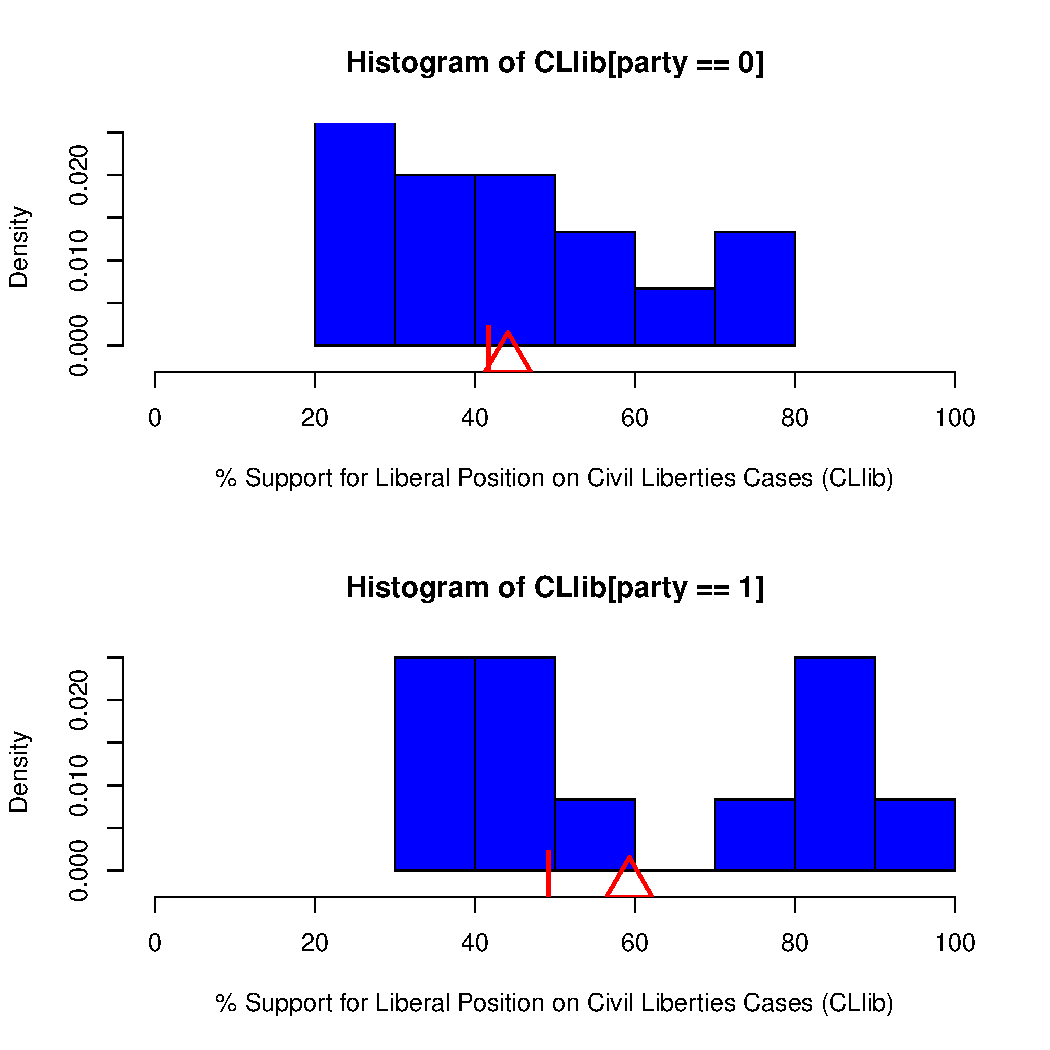
\includegraphics[angle=90,origin=c]{figs/CLhistCond.pdf}}
\end{figure}

}

\frame{
\frametitle{Conditional Mean/Median Discussion}

In pairs, discuss ... 
\begin{enumerate}
\item What do the mean and median represent in the context of the CLib variable for the justices of each party?
\item What does it mean for the mean to be larger for the Democrats than the Republicans? 
\item What does it mean for the difference in means to be larger than the difference in medians?
\end{enumerate}
}

\frame{
\frametitle{Scatterplot Representation}

\begin{figure}[ht] \centering
        \scalebox{.4}{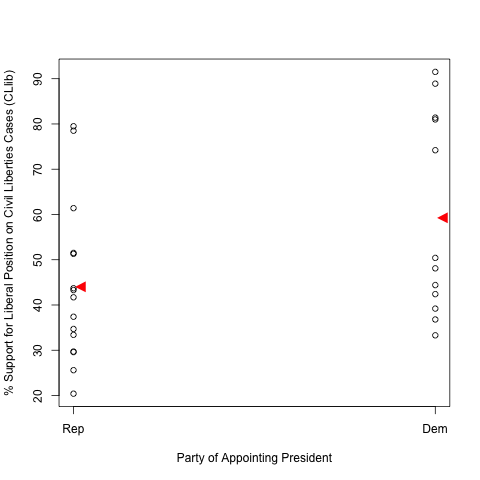
\includegraphics{figs/partyMean.png}}
\end{figure}

}

\frame{
\frametitle{OLS Regression}

\begin{figure}[ht] \centering
        \scalebox{.4}{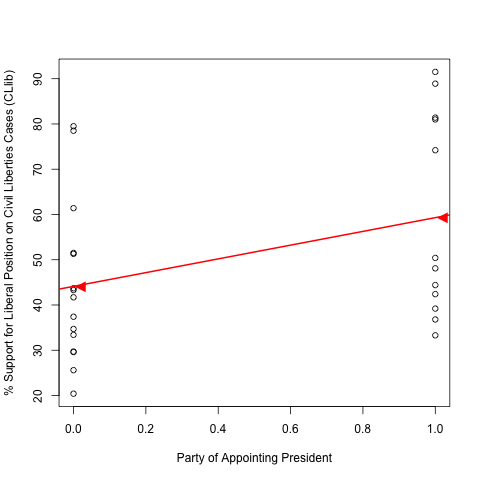
\includegraphics{figs/lmBin.png}}
\end{figure}

}

\frame{
\frametitle{Intercept and Slope Discussion}

In pairs, discuss ... 
\begin{enumerate}
\item The substantive interpretation of the intercept and slope of the line in terms of justices for each party.
\item What does it mean for the mean to be larger for the Democrats than the Republicans? 
\item What does it mean for the difference in means to be larger than the difference in medians?
\end{enumerate}

}

\frame{
\frametitle{Conditional Standard Deviations}

\begin{figure}[ht] \centering
        \scalebox{.4}{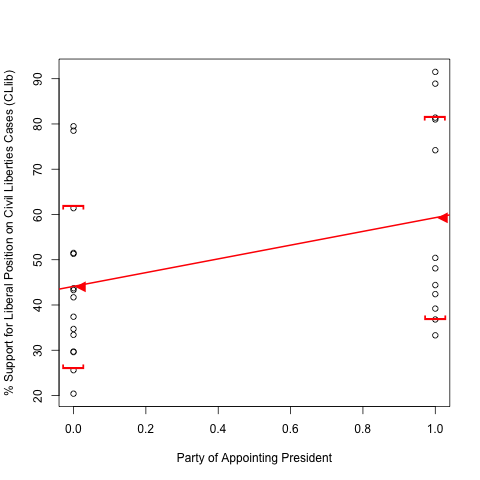
\includegraphics{figs/lmBinSD.png}}
\end{figure}

}

\frame{
\frametitle{Conditional Standard Deviations}

}

\frame{
\frametitle{Special Case: Binary Outcomes}

\begin{itemize}
\item
\end{itemize}

\begin{table}[h]
\begin{center}
\begin{tabular}{r|rr}
Justice & Ur & Party  \\
\hline
Black & 0 & 1 \\
Reed & 0  & 1 \\
\vdots & \vdots \\
Thomas & 1 & 0\\
\hline
\end{tabular}
\end{center}
\end{table}

}

\frame{
\frametitle{Binary Outcome OLS Regression}

\begin{figure}[ht] \centering
        \scalebox{.4}{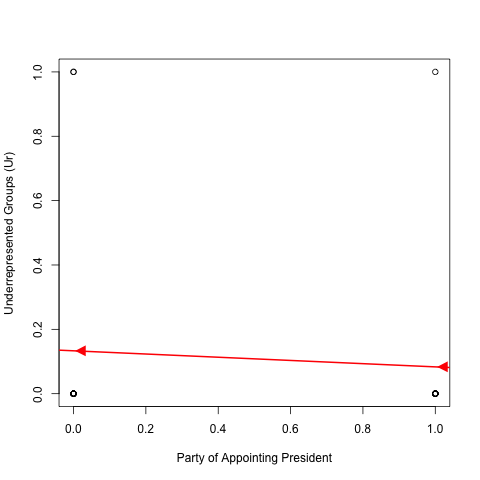
\includegraphics{figs/BinlmBin.png}}
\end{figure}

}

\frame{
\frametitle{Binary Outcome OLS Regression}

\begin{figure}[ht] \centering
        \scalebox{.4}{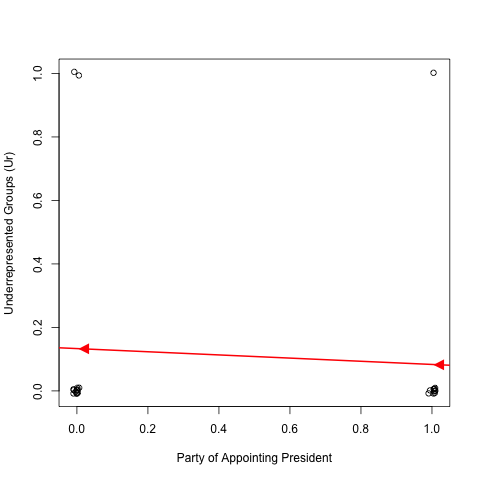
\includegraphics{figs/jitterBinlmBin.png}}
\end{figure}

}





\frame{
\frametitle{Conditional Standard Deviations}

\begin{figure}[ht] \centering
        \scalebox{.4}{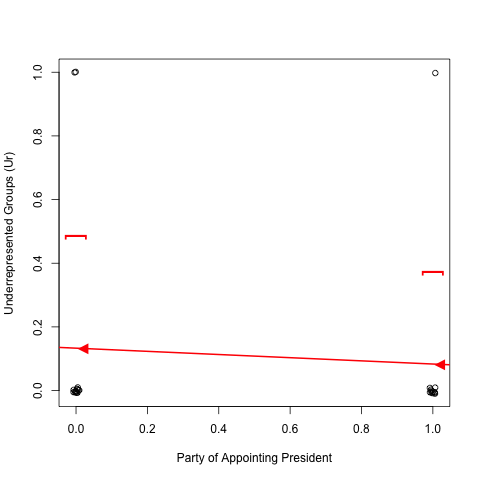
\includegraphics{figs/BinlmBinSD.png}}
\end{figure}

}


\frame{
\frametitle{Binary outcome OLS discussion}

In pairs, discuss ... 
\begin{enumerate}
\item The substantive interpretation of the intercept and slope of the line in terms of justices for each party.
\item Why is the SD smaller for Democrats than Republicans (hint: look at the variance formula for binary variables)
\end{enumerate}

}

\frame{
\frametitle{Summary}

}

\end{document}












